\chapter{Background: Multiview Machine Learning: Concepts, Methods, and Limitations}
\label{chap:background}

\section{Machine Learning}

Machine learning is a branch of artificial intelligence and computer science that focuses on the use of data and algorithms to imitate the way that humans learn, gradually improving its accuracy. Machine learning methods can exploit different forms of supervision signals derived from the data itself, such as contrastive learning, reconstruction, prediction, or clustering. Machine learning methods can also benefit from deep neural networks that can learn expressive and flexible representations from complex and high-dimensional data. Machine learning methods have shown remarkable performance on various tasks, such as computer vision, natural language processing, speech recognition, and recommender systems. The mathematical foundations of Machine learning are provided by mathematical optimization methods.

Machine learning arguably differs from statistics in that it emphasizes the prediction and generalization of out-of-sample data, rather than the explanation and inference of in-sample data. ML methods can handle complex and nonlinear relationships among data, as well as large-scale and high-dimensional data, that may not be suitable for statistical models. Machine learning methods can also learn from unstructured or unlabeled data, such as text or images, that may not have predefined features or categories.

It is common to distinguish between flavours of machine learning based on the type of supervision signal that is used to train the model. Supervised learning methods learn a mapping from inputs to outputs based on a set of training examples and targets. Unsupervised learning methods learn a mapping from inputs to outputs without any training targets. Self-supervised learning methods learn a mapping from inputs to outputs based on a training signal that is derived from the data itself. Reinforcement learning methods learn a mapping from inputs to outputs based on a reward signal that is provided by an environment. In this report we will focus on unsupervised and self-supervised learning methods.

A challenge in machine learning for biomedical applications is that obtaining training data can be expensive and time-consuming. This is particularly true for medical imaging data, which often requires expert annotation. Furthermore, in mental health, there is often a lack of consensus on the definition of a mental health condition, and the boundaries between different conditions are often unclear, even to experts. For this reason, unsupervised and self-supervised learning methods are of particular interest for biomedical applications and will be the focus of this thesis.

\subsection{Unsupervised Learning}

Unsupervised learning methods learn a mapping from inputs to outputs without any training targets. Unsupervised learning methods can be used to learn representations of the data that can be used for downstream tasks such as classification or regression. They can also be used as a way to discover relationships between the data, such as understanding the underlying structure of the data or finding correlations between different modalities of data. Some generative models can also be used to generate new data with similar characteristics to the training data.

Perhaps the most well-known example of unsupervised learning is principal components analysis (PCA), which learns a mapping from inputs to outputs based on the directions of maximum variance in the data. PCA can be used to learn a low-dimensional representation of the data that captures the most variance in the data.

\subsection{Self-Supervised Learning}

Self-supervised learning methods learn a mapping from inputs to outputs based on a training signal that is derived from the data itself. The transformer model behind the success of many Large Language Models (LLMs) such as BERT \cite{devlin2018bert} and GPT-3 \cite{brown2020language} is trained using a self-supervised learning method called masked language modelling. In masked language modelling, the model is trained to predict a masked word in a sentence based on the other words in the sentence. In this case it is clear that . Of closer relevance to this PhD thesis is work on self-supervised learning for computer vision tasks. In these methods, the model is trained to predict a patch of an image based on the other patches in the image.

Like unsupervised learning methods, self-supervised learning methods can be used to learn representations of the data that can be used for downstream tasks such as classification or regression.

\subsection{Multiview Machine Learning}

Throughout this report we will refer to different modalities of data for the same subject as different `views', consistent with the literature\cite{sun2013survey}. Multiview machine learning is a branch of machine learning that deals with data that have multiple sources or modalities that describe the same phenomenon or entity. For example, a person can be represented by their face image, voice, text, and gesture. Each source or modality is referred to as a view, and different views may provide complementary or redundant information.

Multiview learning methods can be used to generate robust low-dimensional representations for a downstream task such as classification or regression, or to discover relationships between views such as correlation or even causation. They been widely applied across a range of fields such as neuroimaging\cite{Krishnan2011}, finance\cite{cassel2000measurement}, Imaging Genetics\cite{Hansen2021}, to find associations between views in large datasets.

Multiview machine learning methods can be interpreted as either unsupervised or self-supervised depending on the context, and this will have important implications for the methods that we will consider in this thesis.

\subsection{Unsupervised Multiview Machine Learning}

Some multiview machine learning models do not treat any of the views as a target. They derive their signal from patterns between the views. For example, in the case of neuroimaging and behavioural data, we may be interested in finding associations between the two views. This is illustrated in figure\ref{fig:mentalhealthsunsupervised}. In this context we can interpret multiview machine learning methods as unsupervised learning methods.

\begin{figure}
    \centering
    \tikz{
        % nodes
        \node[obs, minimum size=2cm] (X_1) {Neuroimage};%
        \node[obs, right=of X_1, minimum size=2cm] (X_2) {Behaviour};%{Behaviour};%
        % edges
        \edge {X_1} {X_2}
        \edge {X_2} {X_1}}
    \caption[Associations between views]{\textit{\textbf{Associations between views:}} From this perspective we identify the strongest associations between neuroimaging modalities and behavioural data which are typically representative of mental health conditions where unhealthy subjects have high variance}
    \label{fig:mentalhealthsunsupervised}
\end{figure}

\subsection{Self-Supervised Multiview Machine Learning}

On the other hand, some multiview machine learning models interpret each view as being an observation of the same underlying object.
Notice that this underlying object could be a latent variable, such as a mental health condition, but it could simply be the subject themselves since each view is an observation of the same subject, Note that these latent variables also need not be categorical, they could be continuous. These latent variables are not observed directly but are inferred from the data. For example, in the case of neuroimaging and behavioural data, the underlying class may be a mental health condition. This is illustrated in figure \ref{fig:mentalhealthselfsupervised} where the latent variable is the severity of some mental health condition and the views are conditioned on this latent variable. In this context we can interpret multiview machine learning methods as self-supervised learning methods.

\begin{figure}
    \centering
    \tikz{
        % nodes
        \node[latent, align=center, minimum size=2cm] (Z) {Severity}; %
        \node[obs, below left=of Z, minimum size=2cm] (X_1) {Neuroimage};%
        \node[obs, below right=of Z, minimum size=2cm] (X_2) {Behaviour};%
        % edges
        \edge{Z} {X_1}
        \edge{Z} {X_2}}
    \caption[Latent Variable Model of Mental Health]{\textit{\textbf{Latent Variable Model of Mental Health:}} From this perspective the neuroimaging modality and behavioural data are both considered to have been generated with distributions conditioned on the severity of a mental health condition}\label{fig:mentalhealthselfsupervised}
\end{figure}

Of particular note for this thesis is that Canonical Correlation Analysis can be interpreted as both an unsupervised (learning associations between views) and a self-supervised (where the derived target is the subject) method depending on the context.

\section{From Principal Components Analysis to Canonical Correlation Analysis}

Canonical Correlation Analysis (CCA)\cite{hotelling1935canonical} is one such multiview machine learning method which has been used to explore the relationships between two or more sets of data by mapping them to a shared unobserved space (`latent variable space') that captures the mutual information across the views. Canonical Correlation Analysis (CCA) and its variants are methods for describing relationships between two or more paired views of the data\cite{uurtio2017tutorial}.

In its original form\cite{hotelling1935canonical}, CCA aims to find linear relationships between the views of data by finding linear orthogonal projections of the data to a latent variable space in which they are maximally correlated. Although educational psychology was one of the first applied uses for CCA, it has found applications in for example natural language processing\cite{dhillon2011multi} and economics\cite{vinod1978survey}. CCA has commonly been effective in neuroimaging tasks such as finding associations between different modalities of neuroimaging or with other measures\cite{wang2018finding}.

In order to explain CCA, it is helpful to first explain the related and arguably simpler principal components analysis (PCA) and partial least squares (PLS) models.

\subsection{Principal Components Analysis}\label{pca}

Principal components analysis (PCA)\cite{hotelling1933analysis} is a method for finding the directions of maximum variance of a matrix $X \in \mathbb{R}^{n \times p}$  where it is common for the rows of $X$ to represent $n$ subjects and the columns $p$ features for each subject. First consider the case $k=2$ where we are interested in the two directions of maximum variance of some data. We show this visually in figure\ref{fig:PCA} for simulated data.

\begin{figure}[H] %[H] "corresponds to start the figure Here" 
    \centering %alignment can be flushleft, centering or flushright
    %includegraphics is the command to include graphics or pictures, [Width should be defined with respect to textwidth]{The path/ location of the image in the specified folder}, the image should be either in .png, .jpg, .pdf formats faster processing
    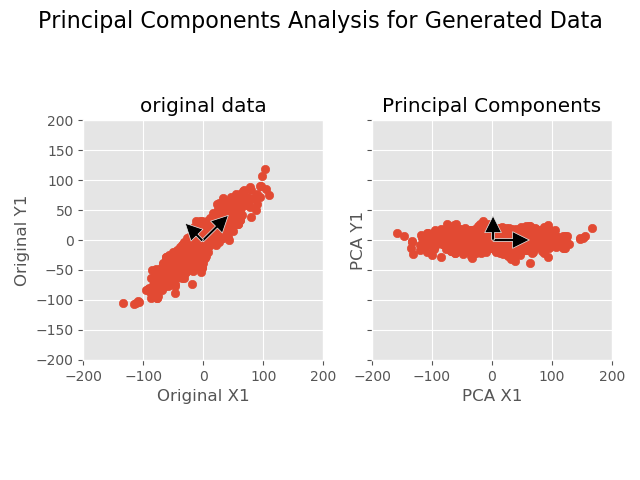
\includegraphics[width=0.9\textwidth]{chapters/2_background/PCA.png}
    \caption[Principal Components Analysis Example]{\textit{\textbf{Principal Components Analysis Example:}} On the left the original data with its directions of maximum variance is shown by the black arrows. On the right we rotate the data to a new basis in which the variance in the direction of the basis is maximised.}\label{fig:PCA}\end{figure}

As we can see, the direction of maximum variance must be a weighted sum of the directions of the feature space which we denote as a vector $w$ (in two dimensions, this gives us a rotation matrix). Since we have defined $w$ as a direction it also has unit length. The variance of the data in that direction will be given by the l2-norm of $Xw$ defined as:

\begin{align}
     & \|Xw\|^2_2=w^{\top}X^{\top}Xw
\end{align}

The equation follows because $Xw$ is a vector of length $N$ with one element for each row of the original data. PCA can therefore be represented by the optimisation problem:

\begin{align}
     & \bold{w_{opt}}=\underset{\bold{w}}{\mathrm{argmax}}\{\bold{w^{\top}X^{\top}}\bold{Xw}\} \\
     & \text{subject to:} \notag                                                               \\
     & \bold{w^{\top}w}=1 \notag
\end{align}

The equation follows because $\bold{Xw}$ is a vector of length $N$ with one element for each row of the original data.

We can write this optimisation problem in its lagrangian form as the function:

\begin{align}
     & f(\bold{w},\lambda)=\bold{w^{\top}X^{\top}}\bold{Xw} + \lambda(1-\bold{w^{\top}w})
\end{align}

Where $\lambda$ is an auxiliary variable called a Lagrange multiplier. A solution to the original optimisation problem must maximise this function with respect to $w$ and also have 0 derivative with respect to $\lambda$ since this results in the equality constraints being fulfilled.

By differentiating the lagrangian function, we find first order conditions which must be satisfied by any solution where the constraints are active:

\begin{align}
     & \bold{X^{\top}}\bold{Xw}=\lambda \bold{w} \\
     & \bold{w^{\top}w}=1
\end{align}

This can now be understood as an eigenvalue problem for the variance-covariance matrix $\bold{X^{\top}X}$ for which we have standard solvers (e.g. scikit-learn in Python\cite{pedregosa2011scikit}). The mathematical intuition behind this form is that the variance-covariance matrix $\bold{X^{\top}X}$ contains the covariance between each pair of variables of $X$ with the variance of each variable on the diagonal. Since this matrix is symmetric, it is also diagonalizable (can be written $\bold{A=P^{-1}DP}$) and the associated eigenvectors would correspond to a change of basis $\bold{P}$ (a rotation matrix). Since by definition the eigenvectors are orthogonal, the diagonal elements must then represent the variance of $\bold{X}$ in each new basis direction and the eigenvectors are orthogonal by definition.

The first principal component is then the direction in which the variance of the data is a maximum or equivalently the eigenvector associated with the maximum eigenvalue $\lambda$. We can find further components by taking the ordered eigenvectors in order of their eigenvalues. If each of the variables in $\bold{X}$ are orthogonal, then it follows that the principal components are simply the direction of each of the original variables, ordered by highest to lowest variance.

In this report, we will typically refer to $w$ as \textbf{weights}, $z=Xw$ as \textbf{projections} or \textbf{latent dimensions}.

In the context of finding relationships between high-dimensional neuroimaging and behavioural modalities, we could reduce the dimensions of both before looking for relationships between them. However the problem with applying PCA to one or both datasets is that it does not account for the variance in the other dataset. This means that by performing dimensionality reduction in one dataset, we may remove the variance that is associated with the other dataset if the useful signal is a small component.

\subsection{Partial Least Squares}

Partial least squares (PLS) is a method for finding the directions of the maximum shared covariance between two paired views of the data. Interestingly, PCA can be seen as a special case of PLS where the two paired datasets are the same. The process is therefore somewhat similar to that in PCA except that we now have two sets of directions and we susbtitute the covariance for the cross-covariance. It can therefore be represented by the optimisation problem:

\begin{align}
     & \bold{w_{opt}}=\underset{\bold{w}}{\mathrm{argmax}}\{ \bold{w_1^{\top}X_1^{\top}X_2w_2}  \} \\
     & \text{subject to:} \notag                                                                   \\
     & \bold{w_1^{\top}w_1}=1 \notag                                                               \\
     & \bold{w_2^{\top}w_2}=1 \notag
\end{align}

Where $\bold{X_1} \in \mathbb{R}^{n \times p_1}$ and $\bold{X_2} \in \mathbb{R}^{n \times p_2}$ or in other words we have two `views' with the same number of subjects but a potentially different number of features.

We can formulate PLS as the solution to an appropriate eigenvalue problem, the singular value decomposition of the covariance matrix $\bold{X_1^{\top}X_2}$, and the solution to an iterative algorithm.

\subsubsection{Eigenvalue Problem}

This has a lagrangian form:

\begin{align}
     & f(w,\lambda)=\bold{w_1^{\top}X_1^{\top}X_2w_2} + \lambda_1(1-\bold{w_1^{\top}w_1}) + \lambda_2(1-\bold{w_2^{\top}w_2})
\end{align}

With first order conditions:

\begin{align}
     & \bold{X_2^{\top}X_1w_1}=\lambda_2\bold{w_2} \\
     & \bold{X_1^{\top}X_2w_2}=\lambda_1\bold{w_1} \\
     & \bold{w_1^{\top}w_1}=1                      \\
     & \bold{w_2^{\top}w_2}=1
\end{align}

By substituting the second two conditions into the first two conditions we find that $\lambda_1=\lambda_2=\lambda$ by symmetry and therefore we can substitute the second into the first condition which becomes:

\begin{align}
     & \bold{X_2^{\top}X_1w_1}=\lambda^2\bold{(X_1^{\top}X_2)^{-1}w_1} \\
     & \bold{X_1^{\top}X_2X_2^{\top}X_1w_1}=\lambda^2\bold{w_1}
\end{align}

And similarly, substituting the first condition into the second:

\begin{align}
     & \bold{X_2^{\top}X_1X_1^{\top}X_2w_2}=\lambda^2\bold{w_2}
\end{align}

Once again, this is the same as finding the eigendecomposition of the matrices $\bold{X_1^{\top}X_2X_2^{\top}X_1}$ and $\bold{X_2^{\top}X_1X_1^{\top}X_2}$. The eigenvectors of the first matrix are then weights $\bold{w_1}$ and the eigenvectors of the second are then weights $\bold{w_2}$. Hoskuldsson showed that the weights and projections of partial least squares can be summarised by four eigenvalue problems \cite{hoskuldsson1988pls}.

\subsubsection{Singular Value Decomposition}

The SVD is a generalization of the eigendecomposition for non square matrices. We can show that finding the eigenvectors from these two eigendecompositions are equivalent to finding the "singular value decomposition" (SVD) of the matrix $X_1^{\top}X_2$ due to the following relationship:

\begin{align}
     & \text{SVD}(\bold{X_1^{\top}X_2})=\bold{U\Sigma V^{\top}}                                                              \\
     & \bold{X_1^{\top}X_2X_2^{\top}X_1}=\bold{U\Sigma (V^{\top} V) \Sigma^{\top} U^{\top}=U(\Sigma \Sigma^{\top}) U^{\top}} \\
     & \bold{X_2^{\top}X_1X_1^{\top}X_2}=\bold{V\Sigma^{\top} (U^{\top} U) \Sigma V^{\top}=V(\Sigma^{\top} \Sigma) V^{\top}}
\end{align}

Using the SVD, the matrix of the left singular vectors $\bold{U}$ are the matrix of weights $\bold{W_1}$ and the matrix of right singular vectors $\bold{V^{\top}}$ are the matrix of weights $\bold{W_2}$.

\subsubsection{Iterative solution with NIPALS}

Since we are typically only interested in the top PLS components, the most common algorithm for solving PLS is the "Nonlinear Iterative Partial Least Squares" (NIPALS) algorithm \cite{wold1966estimation}
which is related to the power method for finding the top components of an SVD and is shown in algorithm \ref{alg:NIPALS}.

\vspace{\baselineskip}
\begin{algorithm}
    \begin{algorithmic}
        \STATE {Finds projections of each view which maximise covariance between the views}
        \STATE $M_1=X_1^{\top}X_2$
        \FOR {$k \gets 1 \textbf{to} K$}
        \STATE {Initialize} $|w^{(k)}_2|_2=1$
        \WHILE {Not converged}
        \STATE $w^{(k+1)}_1=M_kw^{(k)}_2$
        \STATE $w^{(k+1)}_1=\frac{w^{(k+1)}_1}{\|w^{(k+1)}_1\|_2}$
        \STATE $w^{(k+1)}_2=M_k^{\top}w^{(k+1)}_1$
        \STATE $w^{(k+1)}_2=\frac{w^{(k+1)}_2}{\|w^{(k+1)}_2\|_2}$
        \STATE$M_{k+1}=M_k-du_kv_k^{\top}$
        \ENDWHILE
        \ENDFOR
        \caption[NIPALS for PLS]{NIPALS algorithm for PLS}
        \label{alg:NIPALS}
    \end{algorithmic}
\end{algorithm}

The problem with applying PLS to neuroimaging and behavioural modalities is that PLS is not scale invariant and is therefore biased towards the largest principal components in the data \cite{helmer2020stability}. This is particularly problematic when there is a low signal to noise ratio since PLS may find directions in either dataset which correspond to the largest directions of noise in the other.

\subsection{Canonical Correlation Analysis}\label{sec:cca}

Returning to CCA, we now would like to find the directions of maximum correlation rather than of maximum covariance between two views of a dataset. This small change makes CCA invariant to the scale of the features. CCA can therefore be represented by the optimisation problem:

\begin{align}
     & \bold{w_{opt}}=\underset{\bold{w}}{\mathrm{argmax}}\{ \bold{w_1^{\top}X_1^{\top}X_2w_2}  \} \\
     & \text{subject to:} \notag                                                                   \\
     & \bold{w_1^{\top}X_1^{\top}X_1w_1}=1 \notag                                                  \\
     & \bold{w_2^{\top}X_2^{\top}X_2w_2}=1 \notag
\end{align}

Despite this problem being non-convex, the CCA problem has been well studied in the literature and there are a number of other ways of forming and solving the CCA objective. CCA can be formed as an iterative optimisation using an eigenvalue problem, a generalised eigenvalue problem, block coordinate descent by alternating least squares regressions \cite{golub1995canonical} \cite{sun2008least} or by gradient descent \cite{via2007learning}.

\subsubsection{Eigenvalue Problem}

By forming the lagrangian and taking partial derivatives in the same way as the PLS case we have first order conditions:

\begin{align}\label{CCA:FOCs}
     & \bold{X_2^{\top}X_1w_1}=\lambda_2 \bold{X_2^{\top}X_2w_2} \\
     & \bold{X_1^{\top}X_2w_2}=\lambda_1 \bold{X_1^{\top}X_1w_1} \\
     & \bold{w_1^{\top}X_1^{\top}X_1w_1}=1                       \\
     & \bold{w_2^{\top}X_2^{\top}X_2w_2}=1
\end{align}

By again substituting the second two conditions into the first two conditions, we once again have $\lambda_1=\lambda_2=\lambda$. Then substituting the second condition into the first, and recognising $\bold{X_i^{\top}X_i}$ as the covariance matrix of $\bold{X_i}$, $\bold{\Sigma_{ii}}$, and $\bold{X_i^{\top}X_j}$ as the cross-covariance matrix $\bold{\Sigma_{ij}}$, we show that the optimisation problem is another pair of eigenvalue problems:

\begin{align}
     & \bold{X_2^{\top}X_1w_1}=\lambda^2\bold{X_2^{\top}X_2(X_1^{\top}X_2)^{-1}X_1^{\top}X_1w_1}              \\
     & \bold{(X_1^{\top}X_1)^{-1}X_1^{\top}X_2(X_2^{\top}X_2)^{-1}X_2^{\top}X_1w_1}=\lambda^2\bold{w_1}\notag \\
     & \bold{\Sigma_{11}^{-1}\Sigma_{12}\Sigma_{22}^{-1}\Sigma_{21}w_1}=\lambda^2\bold{w_1}\notag             \\
\end{align}

Likewise, we have:

\begin{align}
     & \bold{(X_2^{\top}X_2)^{-1}X_2^{\top}X_1(X_1^{\top}X_1)^{-1}X_1^{\top}X_2w_2}=\lambda^2\bold{w_2}\notag \\
     & \bold{\Sigma_{22}^{-1}\Sigma_{21}\Sigma_{11}^{-1}\Sigma_{12}w_2}=\lambda^2\bold{w_2}\notag             \\
\end{align}

We can also find an alternative form of CCA by reparameterizing $w^*_i=(X_i^{\top}X_i)^{-\frac{1}{2}}w_i$. Then the CCA optimization problem becomes:

\begin{align}
     & \bold{w^*_{opt}}=\underset{\bold{w*}}{\mathrm{argmax}}\{ \bold{w^{*T}_1(X_1X_1^{\top})^{-\frac{1}{2}}X_1^{\top}X_2(X_2^{\top}X_2)^{-\frac{1}{2}}w^*_2\}} \\
     & \text{subject to:} \notag                                                                                                                                \\
     & \bold{w^{*T}_1w^*_1}=1 \notag                                                                                                                            \\
     & \bold{w^{*T}_2w^*_2}=1 \notag
\end{align}

Which we recognise once again as an eigenvalue problem and an associated SVD, this time finding the SVD of $\bold{(X_1X_1^{\top})^{-\frac{1}{2}}X_1^{\top}X_2(X_2^{\top}X_2)^{-\frac{1}{2}}}$ or $\bold{T}=\bold{\Sigma^{-\frac{1}{2}}_{11}\Sigma_{12}\Sigma^{-\frac{1}{2}}_{22}}$. This form of the problem will later form the basis of the Deep Canonical Correlation Analysis (DCCA).

In this form, we can also see that PLS can be made equivalent to CCA by whitening the data matrices prior to forming the covariance matrix (transforming the data covariance to an identity matrix) because this ensures that $\bold{\Sigma^{-\frac{1}{2}}_{ii}}$ is equal to the identity matrix and makes the problem equivalent to PLS. When the number of features exceeds the number of samples $p>n$, CCA degenerates because the within-view covariance matrices cannot be inverted - a major difference between CCA and PLS which can always be computed.

\subsubsection{Generalized Eigenvalue Problems}

Interestingly, we can also set up the system of equations in equation \ref{CCA:FOCs} in matrix form:

\begin{align}
    \begin{pmatrix}
        0                  & \bold{\Sigma_{12}} \\
        \bold{\Sigma_{21}} & 0
    \end{pmatrix}
    \begin{pmatrix}
        \bold{w_1} \\
        \bold{w_2}
    \end{pmatrix}
    =
    \lambda
    \begin{pmatrix}
        \bold{\Sigma_{11}} & 0                  \\
        0                  & \bold{\Sigma_{22}}
    \end{pmatrix}
    \begin{pmatrix}
        \bold{w_1} \\
        \bold{w_2}
    \end{pmatrix}
\end{align}

Which is of the form $\bold{A v} = \lambda \bold{B v}$. CCA is therefore often referred to as a generalized eigenvalue problem for which there are a number of publicly available solvers.

\subsection{Sample Covariance and Population Covariance}
All of the methods can be described through covariance terms: $\mathbb{E}[X^TX]=\Sigma_{XX}$, $\mathbb{E}[Y^TY]=\Sigma_{YY}$, and $\mathbb{E}[X^TY]=\Sigma_{XY}$. We can either consider our training data as samples from the population covariances $\Sigma$ or we can consider the Sample Average Approximation $\frac{1}{b-1}\bar{\mathbf{X}} \bar{\mathbf{Y}}^T=\hat{\Sigma_{XY}}$ where we have a minibatch $b$ of pairs of samples from $X,Y$ into the data matrices $\mathbf{X} \in \R^{p \times b}, \mathbf{Y} \in \R^{q \times b}$ and we let $\bar{\mathbf{X}},\bar{\mathbf{Y}}$ be the centred versions.

\textbf{PCA} is an unsupervised learning algorithm that performs dimensionality reduction by finding new uncorrelated variables that successively maximize variance. These new variables are called principal components and are linear combinations of the original variables. PCA reduces to solving an eigenvalue/eigenvector problem of $\Sigma_{XX}$.

\textbf{LDA} is a supervised learning algorithm that performs dimensionality reduction by finding new variables that maximize the between-class variance while minimizing the within-class variance. These new variables are called linear discriminants and are linear combinations of the original variables. LDA reduces to solving a generalized eigenvalue/eigenvector problem of $\mathbf{S}_B$ and $\mathbf{S}_W$. For LDA, we also need to define the between-class scatter matrix $\mathbf{S}_B$ and the within-class scatter matrix $\mathbf{S}_W$ which in the sample case are:

$$
    \hat{\mathbf{S}_B} = \sum_{i=1}^{c} n_i (\mu_i - \mu)(\mu_i - \mu)^T
$$

$$
    \hat{\mathbf{S}_W} = \sum_{i=1}^{c} \sum_{x \in X_i} (x - \mu_i)(x - \mu_i)^T
$$

\textbf{PLS} is a multiview learning algorithm that performs dimensionality reduction by finding new variables that maximize the covariance between two sets of variables $X$ and $Y$. These new variables are called partial least squares components and are linear combinations of the original variables. PLS reduces to solving an eigenvalue/eigenvector problem of $A=\begin{pmatrix} 0 & \Sigma_{XY} \\ \Sigma_{YX} & 0 \end{pmatrix}$ and $B=I$.

\textbf{CCA} is a multiview learning algorithm that performs dimensionality reduction by finding new variables that maximize the correlation between two sets of variables $X$ and $Y$. These new variables are called canonical components and are linear combinations of the original variables. CCA reduces to solving a generalized eigenvalue/eigenvector problem of $A=\begin{pmatrix} 0 & \Sigma_{XY} \\ \Sigma_{YX} & 0\end{pmatrix}$ and $B=\begin{pmatrix} \Sigma_{XX} & 0 \\ 0 & \Sigma_{YY} \end{pmatrix}$.

\textbf{Multi-view CCA} is a straightforward extension of CCA to the case of 3-or more datasets.
There are various different generalisations of CCA to 3-or-more views in the literature.
But here we describe the most natural GEP-based extension of the two view case. Just write down the relevant $A,B$.
\begin{equation}\label{eq:multi-view-cca-GEV}
    A = \begin{pmatrix} 0 &\Sigma_{XY} & \Sigma_{XZ} \\ \Sigma_{YX} & 0 & \Sigma_{YZ} \\ \Sigma_{ZX} & \Sigma_{ZY} & 0 \end{pmatrix}, \qquad
    B = \begin{pmatrix}\Sigma_{XX} & 0 & 0 \\ 0 & \Sigma_{YY} & 0 \\ 0 & 0 & \Sigma_{ZZ} \end{pmatrix}, \qquad
    w =\begin{pmatrix}	u \\ v \\ w \end{pmatrix}
\end{equation}

Table \ref{tab:subspace} summarizes the definitions of $A$ and $B$ for different subspace learning methods.


%table with PCA, LDA, CCA, PLS and their definitions of A and B e.g. PCA A=X'X B=I.
\begin{table}[h]
    \centering
    \begin{tabular}{|c|c|c|c|}
        \hline
        Method & $A$                                                                                    & $B$                                                                & $W$                                    \\
        \hline
        PCA    & $\Sigma_{XX}$                                                                          & $\mathbf{I}$                                                       & $\begin{pmatrix}W\end{pmatrix}$        \\
        \hline
        LDA    & $\mathbf{S}_B$                                                                         & $\mathbf{S}_W$                                                     & $\begin{pmatrix}W\end{pmatrix}$        \\
        \hline
        CCA    & $\begin{pmatrix} \Sigma_{XX} & \Sigma_{XY} \\ \Sigma_{YX} & \Sigma_{YY} \end{pmatrix}$ & $\begin{pmatrix} \Sigma_{XX} & 0 \\ 0 & \Sigma_{YY} \end{pmatrix}$ & $\begin{pmatrix} U \\ V \end{pmatrix}$ \\
        \hline
        PLS    & $\begin{pmatrix} 0 & \Sigma_{XY} \\ \Sigma_{YX} & 0 \end{pmatrix}$                     & $\mathbf{I}$                                                       & $\begin{pmatrix} U \\ V \end{pmatrix}$ \\
        \hline
    \end{tabular}
    \caption{Definitions of $A$ and $B$ for different subspace learning methods. $\mathbf{S}_B$ and $\mathbf{S}_W$ are the between and within class scatter matrices. With the exception of PLS, $\textbf{A}$ is always positive semi-definite.}
    \label{tab:subspace}
\end{table}

\subsubsection{CCA and PLS vs PCA for Dimensionality Reduction}

It is reasonable at this stage to ask why we would ever use CCA or PLS to learn representations for a downstream task given we already have PCA. An interesting property of CCA is that if noise in the two views is uncorrelated, then the learned representation (which maximises correlation) will not contain the noise regardless of its amplitude. This is in contrast to PCA which could keep all of the uncorrelated noise provided it has sufficiently high variance. On the other hand, CCA will not contain signals which only appear in one of the views. Since CCA removes uncorrelated noise, we may be able to remove some of the measurement noise of traditional diagnostic tools like questionnaires by combining them with neuroimaging or genetic data. Diagnoses based on this latent space could be more robust since the signal they contain must necessarily be supported by both datasets.

\section{Adding regularisation to CCA and PLS}

Regularised solutions to the CCA problem are desirable both to provide a solution in the case where the number of features, $p$ exceeds the number of observations, $n$ as well as to improve the robustness of the projections in the case where we expect noisy observations \cite{branco2005robust} and/or to produce sparse solutions for better interpretability \cite{parkhomenko2009sparse}.

\subsection{Ridge regularisation}\label{sec:Regularised CCA}

Vinod proposed the "Canonical Ridge" which combined the PLS and CCA constraints in a single constrained optimisation \cite{vinod1976canonical}:

\begin{align}
     & w_{opt}=\underset{w}{\mathrm{argmax}}\{\bold{w_1^{\top}X_1^{\top}X_2w_2}\}      \\
     & \text{subject to:} \notag                                                       \\
     & (1-\tau_1)\bold{w_1^{\top}X_1^{\top}X_1w_1}+\tau_1\bold{w_1^{\top}w_1}=1 \notag \\
     & (1-\tau_2)\bold{w_2^{\top}X_2^{\top}X_2w_2}+\tau_2\bold{w_2^{\top}w_2}=1 \notag
\end{align}

Where $\tau_i$ is a mixing hyperparameter that makes the solution more or less CCA-like ($c_i=0$) or PLS-like ($c_i=1$) depending on the constraint. By once again forming the lagrangian and taking partial derivatives we have first order conditions:

\begin{align}
     & \bold{X_1^{\top}X_2w_2} + \lambda_1((1-\tau_1)\bold{X_1^{\top}X_1w_1}+\tau_1\bold{w_1}-1)=0 \\
     & \bold{X_2^{\top}X_1w_1} + \lambda_2((1-\tau_2)\bold{X_2^{\top}X_2w_2}+\tau_2\bold{w_2}-1)=0
\end{align}

And this gives us the eigenvalue problems \cite{rosipal2005overview}:

\begin{align}
     & ((1-\tau_1)\bold{X_1^{\top}X_1}+\tau_1I)^{-1}\bold{X_1^{\top}X_2}((1-\tau_2)\bold{X_2^{\top}X_2}+\tau_2I)^{-1}\bold{X_2^{\top}X_1w_1}=\lambda^2\bold{w_1} \notag \\
     & ((1-\tau_2)\bold{X_2^{\top}X_2}+\tau_2I)^{-1}\bold{X_2^{\top}X_1}((1-\tau_1)\bold{X_1^{\top}X_1}+\tau_1I)^{-1}\bold{X_1^{\top}X_2w_2}=\lambda^2\bold{w_2}
\end{align}

The main difference between this eigenvalue problem and the CCA eigenvalue problem is the substitution of the matrices $\bold{X_1^{\top}X_1}$ and $\bold{X_2^{\top}X_2}$ for the matrices $((1-\tau_1)\bold{X_1^{\top}X_1}+\tau_1I)$ and $((1-\tau_2)\bold{X_2^{\top}X_2}+\tau_2I)$. We can therefore see that this regularisation is equivalent to adding a constant to the diagonal of the covariance matrix $\bold{X_i^{\top}X_i}$. Hardoon showed that this form of regularisation can also be implemented using the kernel trick \cite{hardoon2004canonical}.

\section{Multiple Effects, Orthogonality, and Deflation}\label{sec:orthogonality}

We have only explicitly referred to the vectors of weights that produce maximal variance or correlation so far in this report. However the eigendecomposition formulations of PCA, PLS, and CCA with multiple possible eigenvector and eigenvalue pairs implies that we are able to find more than one orthogonal effect when using all three methods. We refer respectively to the top-$1$ and top-$k$ PLS and CCA problems to distinguish these problems where $k$ refers to the number of effects we wish to find.

While the SVD and eigendecomposition based methods are able to generate all of the latent dimensions at once, they require the inversion of the covariance matrices $\bold{\Sigma_{11}}$ and $\bold{\Sigma_{22}}$ and therefore for very large data have a high computational cost.

However when we use iterative methods we typically compute only the first (i.e. the maximally correlated/covarying effect). If we wish to find further effects, we must define a way to ensure that any other effects we find are different to the first (i.e. the maximally correlated/covarying effect). By a process of deflation we can remove a given effect from our data and repeat the process to find the next top correlated/covarying effect.

To achieve this we need to project the data in a specific way based on orthogonality.

\subsection{Orthogonality}

In their (generalized) eigenvalue problem form, the definition of orthogonality in the PLS and CCA case is given implicitly. In the PLS case the generalized eigenvalue problem:

\begin{align}
    \begin{pmatrix}
        0                  & \bold{\Sigma_{12}} \\
        \bold{\Sigma_{21}} & 0
    \end{pmatrix}
    \bold{w}
    =
    \lambda
    \bold{w}
\end{align}

Implies that the first component $\bold{w_1}$ and the second component $\bold{w_2}$ must have the relationship $\bold{w_{i_1}^{\top} w_{i_2}}=0$. In other words the weight vectors must be orthogonal.

In the CCA case, the generalized eigenvalue problem:

\begin{align}
    \begin{pmatrix}
        0                  & \bold{\Sigma_{12}} \\
        \bold{\Sigma_{21}} & 0
    \end{pmatrix}
    \bold{w}
    =
    \lambda
    \begin{pmatrix}
        \bold{\Sigma_{11}} & 0                  \\
        0                  & \bold{\Sigma_{22}}
    \end{pmatrix}
    \bold{w}
\end{align}

Implies that the first component $\bold{w_1}$ and the second component $\bold{w_2}$ must have the relationship:

\begin{align}
    \bold{w_{i_1}^{\top}\begin{pmatrix}\bold{\Sigma_{11}} & 0 \\0 & \bold{\Sigma_{22}}
                        \end{pmatrix}w^{(2)}}=0
\end{align}

which implies that the projections for each view $\bold{X_iw_i}$ are orthogonal.

However for both CCA and PLS we could also define effects in different ways and indeed the PLS literature contains a number of variants\cite{hoskuldsson1988pls} \cite{wegelin2000survey}. When using iterative methods, we typically use a procedure known as deflation. The deflation step and initialisation of each inner loop forms an algorithmic "outer loop" while the "inner loop" finds the next largest component. There are two common methods for deflation for CCA and PLS described in the literature: Hotelling's deflation and projection deflation.

\subsection{Hotelling's Deflation}
Hotelling's deflation ensures orthogonality of the weight vectors and is typically used for methods based on the power method for the SVD. Hotelling's deflation removes the covariance, $d$, associated with each set of weights:

\begin{align}
     & d = \bold{w^{\top}_1X^{\top}_1X_2w_2}                                        \\
     & \bold{\Sigma^{(i+1)}_{12}}= \bold{\Sigma^{(i)}_{12}} - d\bold{w_1w^{\top}_2}
\end{align}

Hotelling's deflation only ensures orthogonality of the respective weight vectors when $w_1$ and $w_2$ are true singular vectors. For this reason when the problem is regularised, Hotelling's deflation may be suboptimal.

\subsection{Projection Deflation}

Projection deflation projects each dataset into a subspace that is uncorrelated with its first respective projection. It is used to ensure that the projection vectors are orthogonal. This is the method used by Wold's NIPALS algorithm and is also refered to as mode-A deflation or CCA deflation \cite{mackey2009deflation}.

With this method, the projection of each column of $\bold{X}$ in the direction $\bold{Xw}$ is equal to the cross-product of $\bold{Xw}$ with each column of $\bold{X}$ multiplied by the direction: $\frac{\bold{Xw}}{\|\bold{Xw}\|}$.

\begin{align}
     & P(\bold{X})= \frac{\bold{Xw}}{\|\bold{Xw}\|}\bold{w^{\top}X^{\top}X}
\end{align}

We can then find the residual of $\bold{X}$, the variance in $\bold{X}$  that is orthogonal to the first canonical projection. This ensures that the next set of score vectors will be orthogonal to the first.

\begin{align}
     & P^\perp(\bold{X})= \bold{X} - \frac{\bold{Xw}}{\|\bold{Xw}\|}\bold{w^{\top}X^{\top}X} = (I - \frac{\bold{Xw}}{\|\bold{Xw}\|}\bold{w^{\top}X^{\top})X}
\end{align}

\section{Deep CCA}\label{sec:DCCA}
\subsection{Deep Learning}



\section{Datasets}

In the chapters that follow, we will use a combination of simulated datasets, toy datasets and real datasets. This allows us to demonstrate our work in specific circumstances, circumstances with a clear and well understood ground truth and practical applications respectively. We have chosen large neuroimaging datasets with multimodal data since they typically support more interesting signals and also allow us to demonstrate scalability. Here we briefly describe the major real datasets and our hypotheses about them.





